\title{Big Data for Edge Computing}


\author{Albert Zweistein}
\orcid{1234-5678-9012}
\affiliation{%
  \institution{Institute for Plasma Physics in Documentation}
  \streetaddress{P.O. Box 1234}
  \city{Berlin} 
  \state{Ohio} 
  \postcode{123456-12345}
}
\email{trovato@corporation.com}

\author{Gregor von Laszewski}
\affiliation{%
  \institution{Indiana University}
  \streetaddress{Smith Research Center}
  \city{Bloomington} 
  \state{IN} 
  \postcode{47408}
  \country{USA}}
\email{laszewski@gmail.com}


% The default list of authors is too long for headers}
\renewcommand{\shortauthors}{G. v. Laszewski}


\begin{abstract}
This paper provides a sample of a \LaTeX\ document which conforms,
somewhat loosely, to the formatting guidelines for
ACM SIG Proceedings.
\end{abstract}

\keywords{hid000, use up to 5 keywords}


\maketitle

\section{Organization}

The instructions are available at 

\url{https://github.com/cloudmesh-community/hid-sample/blob/master/paper-instructions.md}

It will bring you to a link allowing you to easily download the PDF
version of the instructions. The PDF document is located at 

\url{https://github.com/cloudmesh-community/hid-sample/raw/master/paper-instructions.pdf}


The template is located at

\url{https://github.com/cloudmesh-community/hid-sample/tree/master/paper}


This sample has some advanced features that may not be offered by
other \LaTeX\ frameworks. All of these features are accessible at this
time throug a makefile. These advanced features are optional and
introduce a number of automated tests for the document. Such tests are
executed through a Makefile. Such makefiles can be executed on Linux
or OSX. They are not available on sharelatex. As we have taught you
how to set up a Linux system in class it is part of the leraning
experience that you use that to verify the correctness of your
paper. Alternatively you can set up a docker container and use
that. It will be your responsibility to create such a container or set
up the Linux environment with a \textit{full} version of \LaTeX\ and biber
installed.

The document is organized in a a repository, that needs to be
replicated into your github repository. {\bf Please make sure that all
  filenames and directory names but a README.md are all lower case and
  have no underscore in it. Please make sure they do not contain a
  space in the filename.} We repeat again: Be mindful about the
capitalization of filenames and directory names. We only use lower
case for any file in our directory and we never use spaces or non ASCI
characters. 

IN order for you to most easily compile the paper you will also need
to check out the directory hid-sample that includes the formats. 

Your recommended directories should look like

\begin{verbatim}
~/github/cloudmesh-community/hid-samle
~/github/cloudmesh-community/hid-sp18-000
\end{verbatim}

where 000 the number part of your hid. The two hid directories are
cloned from github. We taught you how to do this and it is a class
goal that you know how to do it. 

In your hid folder you will find, once it is set up the following
directory and files:


We have the following files that you will modify:

\begin{verbatim}
paper/content.tex
paper/report.tex
paper/report.bib
images/README.md
\end{verbatim}

We separated the content from the report format into two different
files, as we found that students in the past manipulated our format to
circumvent our page limitation and artificially increased spacing and
other unnecessary things that we would consider as cheating.
If you

Thus the only file you are allowed to modify is the content.tex file
and the report.bib bibliography file and the images directory in which
you place your images.

Within the text, images and tables are {\bf must} be placed in floats
as discussed in the handbook. You can place them with \verb|[htb]| at
any place in the document. However, we will for the submission force
the placement at the end of the document. You do not have to place
them at the end. Please keep in mind that tables and figurs and
programs that are also to be placed in figures do not count towards
the paper length. Please also be reminded this is not a presentation
and that lengthy enumerations will lead to point deductions. IN case
of questions, consult with the TAs.

\section{Introduction}

Put here an introduction about your topic. 
We just need one sample reference so the paper compiles in \LaTeX\ so we
put it here~\cite{editor00}.

\section{Figures}

In Figure~\ref{f:fly} we show a fly. Please note that because we use
just columwidth that the size of the figure will change to the
columnwidth of the paper once we change the layout to final. Changing
the layout to final should not be done by you. All figures will be
listed at the end.  Please do not use phrases such as \textit{shown in
  the figure below}. Instead use such as shown in Figure~\ref{f:fly}.

\begin{figure}[!ht]
  \centering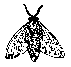
\includegraphics[width=\columnwidth]{../../hid-sample/tex/images/fly.pdf}
  \caption{Example caption}\label{f:fly}
\end{figure}

To avoid copying the example figure in each hid directory, we actually
import it from the hid-sample directory. Lets assume you have a figure
in the image directory called myfigure.pdf. You can than replace the
line in the example with

\begin{verbatim}
\centering\includegraphics[width=\columnwidth]{images/myfigure.pdf}
\end{verbatim}

In case you use png than you must have a png that is at least 300dpi
(find out what that means and how to do that) and use 

\begin{verbatim}
\centering\includegraphics[width=\columnwidth]{images/myotehrfigure.png}
\end{verbatim}

When modifying the example, please do not check in the images from the
examples into your images directory as you will not need them for your
paper. Instead use images that you like to include. If you do not have
any images, do not palce anything in the images folder. However most
technologies could benefit for one image. Make sure you do not
plagiarize the image. Find out from the hand book how to do that. Any
plagiarism of images will result that we return the paper without
review as you have not understood how plagiarism works.

\section{Tables}

In case you need to create tables, you can do this with online tools
(if you do not mind sharing your data) such as
\url{https://www.tablesgenerator.com/} or other such tools (please
google for them). They even allow you to manage tables as CSV.

or generate them by hand while using the provided template in Table
\ref{t:mytable}. Note that
the caption is before the tabular environment.

\begin{table}[htb]
\centering
\caption{My caption}
\label{t:mytabble}
\begin{tabular}{lll}
1 & 2 & 3 \\
\toprule
4 & 5 & 6 \\
7 & 8 & 9
\end{tabular}
\end{table}

\section{Quotes}

Do not use double quotes \verb|"| but use \LaTeX\ ``quotes''. Quotes
{\bf MUST} not be used to highlight works. Quotes are {\bf STRICTLY}
used for quoting text from sources with citation following. If we find
a quote that is not followed by a citation we will return the paper
without review.

\section{Labels}

Do not use actual numbers in the taxt after you write for example
Figure 1 use the ref for the figure while using its label. In our
example it is Figure~\ref{f:fly} and Table Figure~\ref{t:mytabble}.
See the source for the example.

\section{Footnotes}

Footnotes must be avoided in papers. All URLs must be included as full
references and citations and used with the \verb|\cite| command
\footnote{do not use footnotes}. You {\bf must} not use urls in the
text or paper.

\section{Plagiarism}

The class includes a section about plagiarism which you must adhere
to. Copying text without proper citation is considered cheating and we
will assign the grade ``F'' for the paper if we find you do it. It is
in your responsibility to make sure plagiarism does not occur. Please
be aware that our checks are better than the once provided by turnitin
or other online checkers. Excuses such as ``I did not have time'' or
``I forgot'' can not apply as you have enough time to prepare the
paper and must not forget. 

\section{Check}

make sure just as in previous assignments that you check your paper
with chktex and lacheck. Fix the errors that you see. Some of the
errors may be ok, but in general make sure you address all of them. If
in doubt work with the TA. Simply use

\begin{verbatim}
make check
\end{verbatim}

We include in the handbook a list with common issues that we see when
students submit papers. One particular important issue is not to use
the underscore in bibtex labels. It is your responsibility to check
the paper for the issues indicated.

To check bibliographies simply use

\begin{verbatim}
pdflatex report
bibtex report
\end{verbatim}

You will see the errors and warning son the screen address them

TA's will in addition use a special test checking for additional
format issues such as detecting if you used labels and refs for
floats. You are welcome to also try this test, but we provide it
without explanation as no explanation is needed since if you followed
the instructions on floats there should be no issues. If you like to
do that test, you can use  

\begin{verbatim}
make check-ta
\end{verbatim}

\section{Convenient Setup}

If you do not have already a paper dir in your repository, here is a
way to create one. Replace the hid-sp18-000 with your hid.

\begin{verbatim}
export HID=hid-sp18-000
mkdir -p ~/github/cloudmesh-community
cd ~/github/cloudmesh-community
git clone https://github.com/cloudmesh-community/hid-sample.git
git clone https://github.com/cloudmesh-community/$HID.git
\end{verbatim}

Next copy the paper example

\begin{verbatim}
cp -r hid-sample/paper $HID
cd $HID
git add paper
git commit -m "add the paper directory" paper
git push
\end{verbatim}

Make sure there is no \verb|/| behind the paper in the cp command or you mess up the
copy process.


\section{Creating the PDF}

The PDF\ can be created simply with 

\begin{verbatim}
make clean
\end{verbatim}



{\bf UNDER NO CIRCUMSTANCES ARE YOU ALLOWED TO CHECK IN YOUR PDF OR
  TEMPORARY LATEX FILES INTO GITHUB. GIT NEEDS TO STAY CLEAN AND ONLY
  CONTAIN THE SOURCES.}

We will deduct points if you do violate this.

\section{Conclusion}

Put here an conclusion. Conclusion and abstracts must not have any
citations in the section.


\begin{acks}

  The authors would like to thank Dr.~Gregor~von~Laszewski for his
  support and suggestions to write this paper.

\end{acks}

\bibliographystyle{ACM-Reference-Format}
\bibliography{report} 

